\subsection{Cache Correctness and Repair Cost}
\label{sec:eval-kv}

We next ask whether boundary-aware KV repair is necessary for correctness, and whether it remains cheap enough to preserve the first post-promotion user interaction. We separate these two questions explicitly: correctness on the newly appended span after a promotion, and request TTFT on the first post-promotion turn. Exact per-model values and normalized repair work are reported in Appendix~\ref{app:kv-repair-details}.

\paragraph{Methodology.}
For correctness, we use the lossless three-turn probe from Section~\ref{sec:kv_reconcile}. Stage~1 serves span \(A\). After the Stage~\(1\!\rightarrow\!2\) promotion, we append span \(B\) and measure perplexity only on \(B\). After the Stage~\(2\!\rightarrow\!3\) promotion, we append span \(C\) and measure perplexity only on \(C\). We compare three policies: \textit{Oracle-Recompute}, which invalidates the prefix cache and recomputes the prefix under the promoted model; \textit{Stale-Reuse}, which reuses pre-promotion KV unchanged; and \textit{ProgressiveServe-Repair}, which preserves the unchanged lower-prefix state and rematerializes only the suffix at and beyond the promotion point. To avoid ratio-heavy presentation, we report \(\Delta\)PPL relative to \textit{Oracle-Recompute}.

\paragraph{Repair is required for correctness.}
Figure~\ref{fig:kv-delta-ppl} shows a consistent pattern across LLaMA-2-7B, Falcon-7B, Gemma-7B, and LLaMA-2-13B. \textit{ProgressiveServe-Repair} stays close to the oracle, with \(\Delta\)PPL between \(-0.50\) and \(+0.60\) across both promotions. In contrast, \textit{Stale-Reuse} always degrades correctness: on span \(B\), it adds \(+1.03\) to \(+2.76\) PPL, and on span \(C\), it adds \(+1.43\) to \(+6.79\) PPL. For the representative LLaMA-2-7B run, stale reuse increases PPL by \(+1.74\) on \(B\) and \(+3.87\) on \(C\), whereas ProgressiveServe-Repair stays within \(-0.17\) and \(+0.02\). These gaps are too large to treat stale upper-layer KV as a harmless approximation; once the model changes at promotion time, the affected suffix must be repaired.

\paragraph{Repair keeps the first post-promotion turn responsive.}
Correctness alone would not be useful if repair simply replaced stale reuse with a full-prefix stall. We therefore sweep accumulated prefix length \(T\) in representative LLaMA-2-7B origin-first true end-to-end runs and compare \textit{ProgressiveServe-Repair} against a correctness-preserving \textit{Full-Reset} baseline, which discards the prefix cache and forces the next request to re-prefill under the promoted model. Figure~\ref{fig:kv-request-ttft} shows that \textit{Full-Reset} grows sharply with prefix length, while \textit{ProgressiveServe-Repair} remains nearly flat. At \(T{=}1500\), the first post-promotion request TTFT falls from \(227.7\) to \(56.7\) ms for Stage~\(1\!\rightarrow\!2\) and from \(228.5\) to \(54.4\) ms for Stage~\(2\!\rightarrow\!3\). The same trend holds across the full model set at each model's longest tested prefix: ProgressiveServe reduces first-request TTFT by \(171.0\) to \(326.6\) ms while keeping the repair fast path successful in all completed runs.

\paragraph{Takeaway.}
Boundary-aware KV repair is not an optional optimization layered on top of progressive serving. It is required to recover oracle-level post-promotion behavior on the newly appended span, yet it does so without introducing a user-visible full-prefix stall. ProgressiveServe therefore preserves both semantic correctness and request responsiveness across stage promotions.

\begin{figure*}[t]
\centering
\begin{minipage}[t]{0.49\textwidth}
\centering
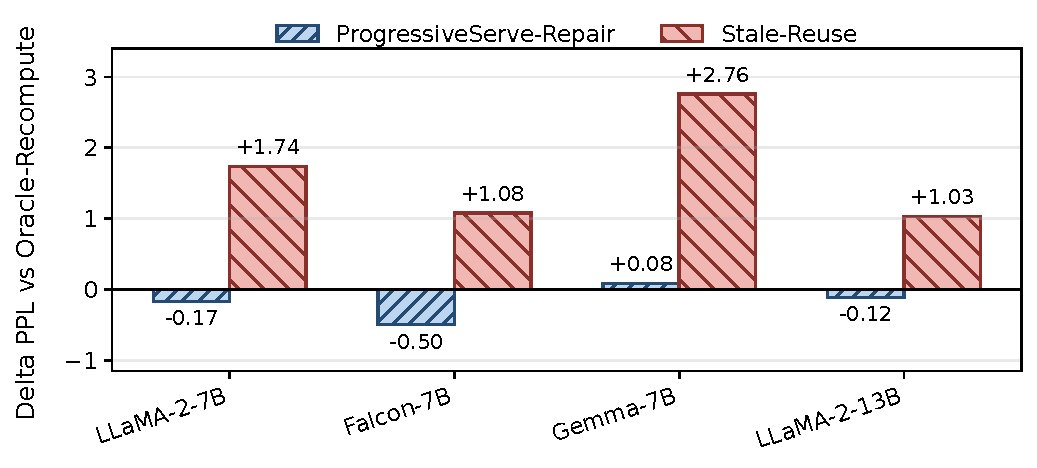
\includegraphics[width=\textwidth]{figures/kv_delta_ppl_stage12_revision.pdf}
\vspace{1mm}

\small\textbf{(a)} \(\Delta\)PPL on span \(B\) after Stage~\(1\!\rightarrow\!2\)
\end{minipage}\hfill
\begin{minipage}[t]{0.49\textwidth}
\centering
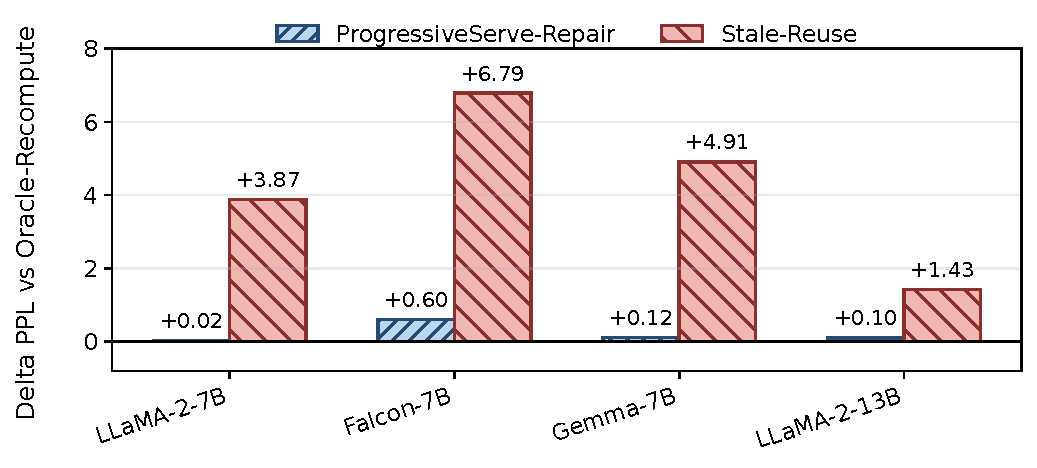
\includegraphics[width=\textwidth]{figures/kv_delta_ppl_stage23_revision.pdf}
\vspace{1mm}

\small\textbf{(b)} \(\Delta\)PPL on span \(C\) after Stage~\(2\!\rightarrow\!3\)
\end{minipage}
\caption{
Cross-model KV-cache correctness reported as \(\Delta\)PPL relative to \textit{Oracle-Recompute}. Models are ordered consistently as LLaMA-2-7B, Falcon-7B, Gemma-7B, and LLaMA-2-13B. The split-panel layout keeps labels readable, and the hatch patterns remain distinguishable even in grayscale print: forward-slash for \textit{ProgressiveServe-Repair} and backslash for \textit{Stale-Reuse}. \textit{ProgressiveServe-Repair} stays near zero across both promotions, while \textit{Stale-Reuse} consistently increases perplexity on the newly appended span.
}
\label{fig:kv-delta-ppl}
\end{figure*}

\begin{figure*}[t]
\centering
\begin{minipage}[t]{0.49\textwidth}
\centering
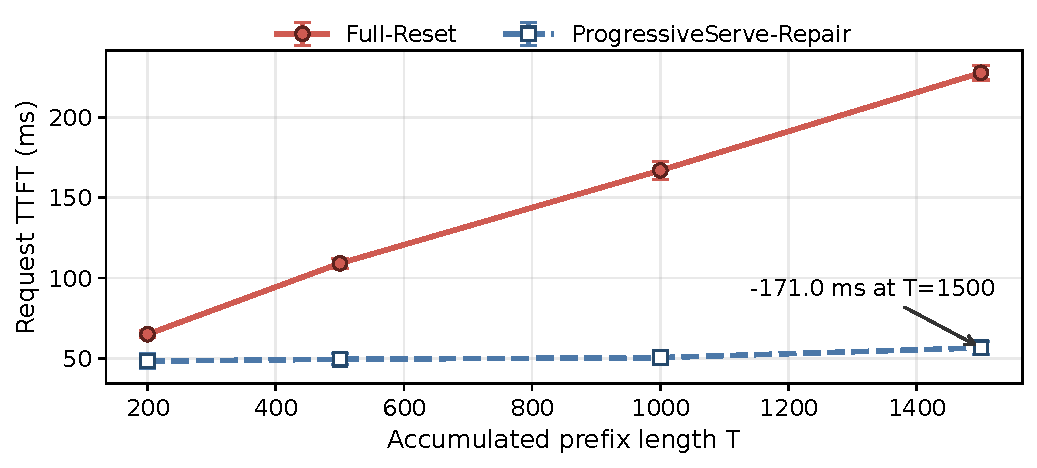
\includegraphics[width=\textwidth]{figures/kv_request_ttft_stage12_revision.pdf}
\vspace{1mm}

\small\textbf{(a)} First post-promotion request TTFT after Stage~\(1\!\rightarrow\!2\)
\end{minipage}\hfill
\begin{minipage}[t]{0.49\textwidth}
\centering
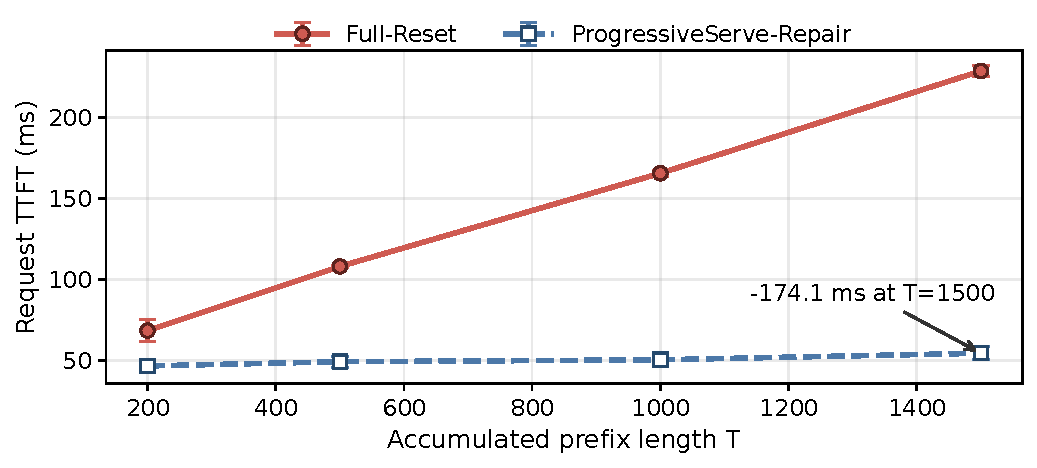
\includegraphics[width=\textwidth]{figures/kv_request_ttft_stage23_revision.pdf}
\vspace{1mm}

\small\textbf{(b)} First post-promotion request TTFT after Stage~\(2\!\rightarrow\!3\)
\end{minipage}
\caption{
First post-promotion request TTFT versus accumulated prefix length \(T\) for representative LLaMA-2-7B origin-first true end-to-end runs. We render the two promotions as separate panels rather than a pre-composed PDF so that each panel can use larger fonts and cleaner annotation placement. \textit{Full-Reset} uses a solid circle-marked line, whereas \textit{ProgressiveServe-Repair} uses a dashed square-marked line. \textit{Full-Reset} incurs a growing full-prefix penalty as \(T\) increases, whereas \textit{ProgressiveServe-Repair} remains nearly flat for both promotions.
}
\label{fig:kv-request-ttft}
\end{figure*}
